\documentclass[tikz,border=2pt]{standalone}
\usepackage{tikz}
\usetikzlibrary{arrows.meta,positioning}
\begin{document}
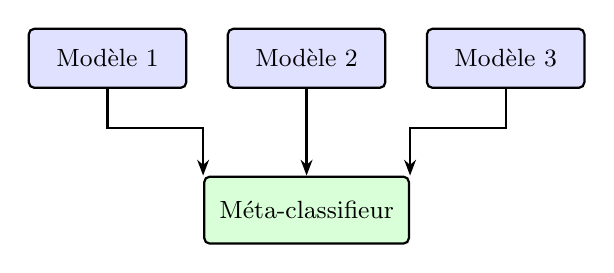
\begin{tikzpicture}[
    font=\small,
    >=Stealth,
    base/.style={draw, thick, rounded corners=2pt, minimum width=2cm, minimum height=0.75cm, align=center},
    meta/.style={draw, thick, fill=green!15, rounded corners=2pt, minimum width=2.6cm, minimum height=0.85cm, align=center}
]
\node[base, fill=blue!12] (m1) {Mod\`ele 1};
\node[base, fill=blue!12, right=0.5cm of m1] (m2) {Mod\`ele 2};
\node[base, fill=blue!12, right=0.5cm of m2] (m3) {Mod\`ele 3};
\node[meta, below=1.1cm of m2] (meta) {M\'eta-classifieur};
\draw[thick, -{Stealth[length=2mm]}] (m1.south) -- ++(0,-0.5) -| (meta.north west);
\draw[thick, -{Stealth[length=2mm]}] (m2.south) -- (meta.north);
\draw[thick, -{Stealth[length=2mm]}] (m3.south) -- ++(0,-0.5) -| (meta.north east);
\end{tikzpicture}
\end{document}
